\section{Giới thiệu}
\subsection{Bài toán Cắt Tấm (Cutting Stock Problem)}

\hspace{0.5cm}Bài toán cắt vật liệu (CSP) là một bài toán tối ưu quen thuộc trong lĩnh vực nghiên cứu vận hành, tập trung vào cách cắt các tấm nguyên liệu lớn thành các mảnh nhỏ hơn nhằm đáp ứng nhu cầu cụ thể và giảm thiểu lãng phí. Bài toán này rất phổ biến trong các ngành công nghiệp như thép, giấy, dệt may, và kính, nơi nguyên liệu thường có kích thước tiêu chuẩn và cần được cắt theo yêu cầu sản xuất. CSP giúp tối ưu hóa việc sử dụng nguyên liệu, giảm chi phí sản xuất và nâng cao hiệu quả vận hành.

Bài toán này được nhà kinh tế học người Nga Leonid Kantorovich lần đầu tiên đề xuất vào năm 1939 \cite{benamor_cutting_2024}. Đến thập niên 1960, Gilmore và Gomory \cite{benamor_cutting_2024} đã giới thiệu kỹ thuật sinh cột (column generation), giúp giải bài toán cắt tấm một chiều hiệu quả hơn bằng cách tạo ra các mẫu cắt dần dần thay vì giải toàn bộ bài toán cùng lúc. Phương pháp này đã tạo nền tảng cho nhiều kỹ thuật hiện đại.

CSP thường được phân loại dựa trên số chiều và sự đa dạng của nguyên liệu và sản phẩm cần cắt. Với độ phức tạp tính toán cao, CSP thuộc loại bài toán NP-hard \cite{IR}, khiến việc tìm lời giải chính xác trở nên không khả thi trong thời gian hợp lý đối với các bài toán lớn. Vì vậy, nhiều thuật toán và phương pháp gần đúng đã được phát triển.

Nhờ tính ứng dụng cao và khả năng tiết kiệm chi phí đáng kể, CSP vẫn là chủ đề nghiên cứu quan trọng. Các phương pháp hiện đại tích hợp các tiến bộ như kỹ thuật sinh cột, nhánh và cận, và cả học máy, đảm bảo ngành công nghiệp liên tục cải thiện hiệu quả và giảm thiểu lãng phí.

\subsection{Bài toán Cắt Tấm Hai Chiều (Two-Dimension Cutting Stock Problem)}

\hspace{0.5cm}Bài toán cắt tấm hai chiều (2DCSP) là một bài toán tối ưu tổ hợp phức tạp, có vai trò quan trọng trong các ngành công nghiệp như sản xuất, hậu cần, và gia công vật liệu. Mục tiêu của 2DCSP là cắt các mảnh nhỏ từ một nguyên liệu lớn hơn, chẳng hạn như tấm hoặc cuộn, đồng thời giảm thiểu lượng vật liệu bị lãng phí. Bài toán này rất phức tạp do phải cân nhắc yếu tố hình học và tối ưu hóa các mẫu cắt, vốn thay đổi tùy theo hình dạng và phương pháp cắt được sử dụng.

Bài toán 2DCSP được phân loại dựa trên loại hình dạng cần cắt, từ các hình dạng đơn giản như hình chữ nhật và hình tròn cho đến các hình dạng phức tạp và không đều. Mỗi loại hình dạng đều mang đến những thách thức riêng trong việc sắp xếp và cắt từ nguyên liệu hiện có.

Hai kỹ thuật cắt chính thường được sử dụng trong 2DCSP là Cắt kiểu guillotine (guillotine cutting) và Cắt không kiểu guillotine (non-guillotine cutting)

\begin{itemize}
    \item Cắt Kiểu Guillotine: Trong phương pháp này, quá trình cắt bị giới hạn bởi các đường cắt thẳng, kéo dài toàn bộ chiều dài hoặc chiều rộng của nguyên liệu. Mỗi đường cắt được thực hiện từ một cạnh của vật liệu đến cạnh đối diện, và các đường cắt này chia nguyên liệu thành các phần nhỏ hơn. Cắt kiểu guillotine đơn giản hóa bài toán bằng cách giảm số lượng mẫu cắt có thể có, nhưng có thể dẫn đến các giải pháp không tối ưu đối với một số cấu hình hình dạng nhất định.
    \begin{figure}[!htp]
        \centering
        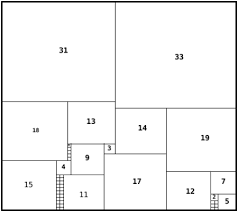
\includegraphics[width=0.25\linewidth]{Images/2dcspgui.png}
        \caption{Minh họa quá trình cắt kiểu Guillotine: Các đường cắt thẳng từ một cạnh đến cạnh đối diện}
        \label{fig:2dcspgui}
    \end{figure}

    \item Cắt Không Kiểu Guillotine: Phương pháp này cho phép linh hoạt hơn trong việc lựa chọn các đường cắt, có nghĩa là cắt có thể thực hiện ở bất kỳ góc độ nào và không bị giới hạn phải cắt qua toàn bộ vật liệu. Mặc dù tính linh hoạt này mang lại cơ hội tối ưu hóa các mẫu cắt hiệu quả hơn, nhưng nó cũng làm tăng độ phức tạp của bài toán, vì có nhiều cấu hình tiềm năng cần xem xét.

    \begin{figure}[!htp]
        \centering
        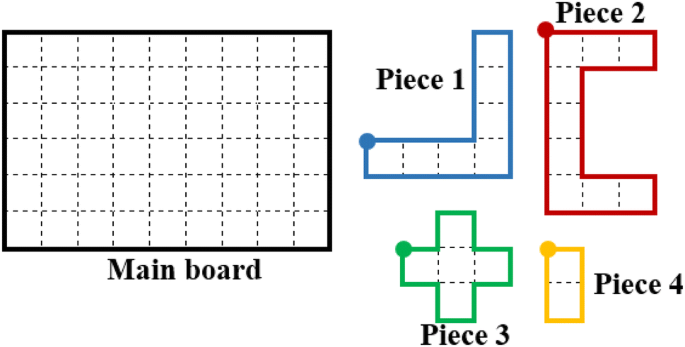
\includegraphics[width=0.5\linewidth]{Images/nongui2dcsp.png}
        \caption{Bài toán cắt tấm hai chiều không kiểu Guillotine}
        \label{fig:enter-label}
    \end{figure}
    
\end{itemize}

Tác động của việc lựa chọn giữa phương pháp cắt kiểu guillotine và không kiểu guillotine là rất lớn. Cắt kiểu guillotine đơn giản hơn khi thực hiện và thường nhanh hơn, nhưng có thể dẫn đến việc lãng phí vật liệu cao đối với các hình dạng không đều hoặc không phải hình chữ nhật. Trong khi đó, cắt không kiểu guillotine cung cấp nhiều cơ hội tối ưu hóa hơn nhưng với cái giá là tăng độ phức tạp tính toán.

Bài toán 2DCSP cũng có ứng dụng rộng rãi trong các tình huống thực tế như sản xuất đồ nội thất, cắt vải, và thậm chí trong thiết kế các bố cục tối ưu cho bảng mạch in (PCBs). Trong tất cả các trường hợp này, mục tiêu vẫn là: giảm thiểu lãng phí và tối đa hóa việc sử dụng nguyên liệu có sẵn, đây là một thách thức quan trọng đòi hỏi việc phát triển các mô hình toán học tinh vi và các thuật toán gần đúng.

\subsection{Cấu trúc bài báo cáo}

\hspace{0.5cm}Nghiên cứu này đóng góp vào bài toán cắt tấm hai chiều (2DCSP) bằng cách giải quyết cả lý thuyết và thực tiễn. Bắt đầu với mô hình toán học ILP, nghiên cứu đánh giá các phương pháp heuristic như Tham lam (Greedy) và Phân bổ Tốt Nhất (Best-Fit), cùng các phương pháp tiên tiến như Tạo Cột (Column Generation). Tính thực tiễn được minh chứng qua nghiên cứu tình huống, áp dụng vào quản lý tài nguyên và cắt bảng mạch in, giúp giảm lãng phí và nâng cao hiệu quả vật liệu. So sánh các thuật toán dựa trên các chỉ số như sử dụng vật liệu và hiệu quả tính toán, nghiên cứu cung cấp cái nhìn về ưu điểm và sự đánh đổi. Cuối cùng, nghiên cứu hướng tới việc tích hợp AI, metaheuristics và ứng dụng trong các lĩnh vực mới như sản xuất gia công bổ sung và hậu cần, đóng góp vào sự phát triển bài toán 2DCSP trong tối ưu hóa công nghiệp.